\documentclass[a4paper, onecolumn, 12pt]{article}
\usepackage[a4paper, total={6in, 8in}]{geometry}
\usepackage[english]{babel}
\usepackage[protrusion=true,
            expansion=true,
            final,
            babel
                ]{microtype}
\usepackage{graphicx} % Required for inserting images
\usepackage{setspace}
\usepackage{parskip}
\usepackage{amsmath}
\usepackage{amssymb}
\usepackage{hyperref}
\usepackage{float}

\hypersetup{
    colorlinks=true,
    linkcolor=blue,
    citecolor=red,
    filecolor=magenta,      
    urlcolor=cyan,
    pdftitle={Overleaf Example},
    pdfpagemode=FullScreen,
}
    
\begin{document}
\graphicspath{{./images}}

\begin{center}
    \doublespacing
    {\Large \textbf{King Fahd University of Petroleum and Minerals} }\\ 
    {\large \textbf{
    College of Computing and Mathematics\\
    Mathematics Department 
    } } 
\end{center} 

\begin{figure}[h]
    \centering
    
\includegraphics[width=200px]{KFUPM_LOGO}
\end{figure}

\begin{center}\onehalfspacing
    \Large \textbf{Math 619-Project}\\
    \normalsize \textbf{Term 231} \\
    \Large \textbf{Progress Report}\\
    \textbf{Project}: Deep Learning Methods for Partial Differential Equations (PDEs)
\end{center}
\vspace{1em}
\large
\begin{center}
\bgroup
\def\arraystretch{1.3}
\begin{tabular}{|c|c|}
    \hline
    \textbf{Name} & \textbf{KFUPM ID} \\
    \hline
    Hashim Al-Sadah & 201578370\\
    \hline
    Abdulwahab Alghamdi & 201734070\\
    \hline
    Hussain Al-Sinan & 202205120\\
    \hline 
\end{tabular}
\egroup
\end{center}
\vspace{1em}
\begin{center}
    \textbf{Instructor:} Dr. Jamal Al-Smail
\end{center}
\normalsize


\onehalfspacing % for double spacing, comment if ypu don't want to
\section*{Abstract}
Partial differential equations (PDEs) are essential components for modelling different processes 
and systems in various scientific and engineering areas. To predict the behavior of a certain system, 
one needs to solve or simulate the PDEs that describe that system. However, 
obtaining an analytical solution to PDEs is a difficult task in most practical situations, 
especially in the case of nonlinear or high dimensional PDEs. 
Due to the rapid evolution and advancements in the field of deep learning, 
researchers are starting to use deep neural networks (DNN) to approximate the solution of PDEs. 
Different models have been developed to perform this task such as Physics-Informed Neural Networks (PINNs) 
and Neural Operator. The speed and the efficiency of these models can surpass other common solvers 
such as Finite Elements (FM), Finite Difference (FD), and spectral methods in certain cases. 
In this project, we will utilize these deep learning models to solve an industry-related problem that 
requires PDEs approximation and compare the accuracy of the used method against 
experimental or simulated data obtained through other available solvers.

\section{Introduction}
Due to the increase power of computation and the success of deep learning models to 
solve different problems in various fields such
as computer vision\cite{chai2021deep}, pattern recognition\cite{serey2023pattern}, 
and natural language and speech processing\cite{NLPChai}, 
researchers were inspired to apply deep neural network to solve problems in the field of scientific computing. 
One of the common and challenging problems is the problem of solving partial differential equations (PDEs).
Different systems and processes are modelled by PDEs whether it is a natural system such as 
modelling a biological or a physical phenomena\cite{grossmann2023can,beck2020overview}, or whether it is not a natural system such as
simulating socioeconomic or financial models\cite{beck2020overview}. Deep learning-based PDEs solver surpass classical methods such as 
finite element or finite difference in certain cases\cite{grossmann2023can}. 
One of them is the case of high dimensional PDEs since classical solvers require discretizing the PDEs' domain into a mesh, 
which causes the number of computations to increase exponentially with the increase of the dimensions and this is known as the curse of dimensionality. 
On the other hand, deep learning models are mesh-free models, and they only require training data from the PDEs domain. 
Other situations where deep neural networks exceeds the traditional solvers is when the PDE is 
nonlinear or non-smooth, which makes it difficult to discretize\cite{grossmann2023can}. 

Physics-informed Neural Network (PINN) is the most basic and widely used model for approximating PDEs' solutions. 
PINN is unsupervised learning model since it does not require any 
labelled data to learn the approximated function or solution\cite{cuomo2022scientific}.
Despite being unsupervised technique, it is possible to include experimental data along with the physical prior knowledge
in order to guide the neural network to the optimal approximation by reducing the 
number of admissible solutions to the problem\cite{hao2022physics,raissi2019physics}.
Similar to the fully connected neural network, the physics-informed neural network consists of 
an input layer, hidden layers, and an output layer. First, the input layer is used to feed 
the training data into the neural network.  Then, the hidden layers map the data to higher dimensions though 
a series of linear transformation followed by a nonlinear activation function. 
Finally, the hidden layers map the data to the output layer, which provides the output of the approximated function. 
The physics-informed neural network (PINN) updates the learning parameters by minimizing a loss function that takes 
into account the losses due the boundary and initial conditions as well as the PDEs' residual. 
After the training process, the neural network should be able to approximate a function that obeys the laws provided by the PDEs. 
Therefore, the procedure of including the PDEs' residual helps to restrict the number of possible solutions\cite{cuomo2022scientific}. 

Another famous model, which has been developed recently, is the Neural Operator model. 
What makes neural operators different from physics-informed neural networks (PINNs) is that the former 
learns a mapping between infinite function spaces unlike PINN where the mapping occurs between finite spaces or sets. 
This enables neural operators to learn an operator instead of a function and hence the name Neural Operator.
The key difference between PINN and neural operators in terms of architecture is that the 
hidden layers in neural operators consist of linear operators, usually integral operators, 
followed by a nonlinear activation function. 
Therefore, neural operators are considered a generalization of physics-informed neural network\cite{kovachki2021neural}.

Overall, deep learning methods for PDEs are powerful solvers. 
They have the potential for resolving various problems and challenges faced by the classical methods. 
The advantage of neural networks models is that they are mesh-free methods, which enables them to approximate 
the solution for nonlinear, non-smooth, and high dimensional PDEs without suffering from the cures of dimensionality.
Furthermore, they utilize the algorithm of automatic differentiation to compute the residual of the PDEs. 
The algorithm is implemented by the majority of deep learning libraries, 
which makes the overall implementation process simple and easy. 

\section{PINN}
In this section, we develop some mathematical notation to use throughout the project, 
and discuss the procedure of approximating ordinary and partial differential equations. All the 
codes that have been used in this section will be available on the GitHub repository 
\url{https://github.com/HashimAlSadah/MX-Project.git}.

Let us first consider a general nonlinear differential equation
\begin{align}
\mathcal{F}(u, \gamma)(\mathbf{x}) = f(\mathbf{x}) \qquad \mathbf{x} \in  \Omega,\\
\mathcal{B}(u, \gamma)(x, t) = g(t) \qquad x \in \partial{\Omega}, \\
\mathcal{I}(u, \gamma)(x, t_0) = h(x) \qquad x \in \partial{\Omega_0}
\end{align}

Where $u(\mathbf{x})$ is the unknown function that we are trying to approximate, 
$\mathbf{x} = [ x_1, x_2, \dots, x_{d-1}, t]$ is the vector of space and time 
in the domain $\Omega \subset \mathbb{R}^d$  with boundary $\partial{\Omega}$, 
$\gamma$ are parameters related to the problem, $\mathcal{F}$ is the nonlinear 
differential operator, $\mathcal{B}$ is the boundary conditions, $\mathcal{I}$ is 
the initial conditions, and $f(\mathbf{x})$, $g(t)$, and $h(x)$ are specified 
functions for a certain problem. 

Since it is established that multilayer feedforward neural networks 
are universal function approximators\cite{hornik1989multilayer}, it means that 
a neural network with at least one hidden layer can approximate a function 
from a finite dimensional set to another with 
any arbitrary error given that we use a sufficient number of hidden neuron or units.
Therefore, the target function $u(\mathbf{x})$ can be approximated with a neural network,
$$
u_{\theta}(\mathbf{x}) \approx u(\mathbf{x})
$$ 
Where $\theta$ represents the parameters of the neural network, which consists of
weights and the biases.

As stated earlier, a neural network is composed of input layer, 
hidden layers, and output layer. Therefore, neural network with $L$
layers can represent $u_\theta$ as a compositional function as the following.
$$
u_{\theta}(\mathbf{x}) = f_L(\mathbf{x}) \circ f_{L-1}(\mathbf{x}) \circ \dots \circ f_1(\mathbf{x})
$$
But each layer consists of a linear transformation and a nonlinear scalar activation function
$$
f_i(\mathbf{x}) = \sigma_i \left( \mathbf{W}_i \cdot \mathbf{x}_i + \mathbf{b}_i \right), 
$$
Denote the linear transformation by $T(\mathbf{x})$
$$
T(\mathbf{x}) = \mathbf{W}_i \cdot \mathbf{x}_i + \mathbf{b}_i 
$$
Therefore, 
\begin{equation}
u_{\theta}(\mathbf{x}) = T_L \circ \sigma \circ T_{L-1} \circ \dots \circ \sigma \circ T_1
\end{equation}
We are assuming that the same activation function $\sigma$ is used for all the layers.

PINN converts the problem of solving a differential equation 
to an optimization problem since PINN attempts to determine the parameters $\theta$ 
that approximate the function $u$ by minimizing a loss function $\mathcal{L}(\theta)$\cite{cuomo2022scientific}.

The loss function includes the partial differential equation, initial and boundary conditions, and 
the labeled data if available.
\begin{equation}
\mathcal{L}(\theta) = w_{\mathcal{F}} \mathcal{L}_{\mathcal{F}}(\theta)
+ w_{\mathcal{B}} \mathcal{L}_{\mathcal{B}}(\theta) 
+ w_{\mathcal{I}} \mathcal{L}_{\mathcal{I}}(\theta)
+ w_{\mathcal{D}} \mathcal{L}_{\mathcal{D}}(\theta)
\end{equation}
Where $\mathcal{L}_{\mathcal{F}}(\theta)$, $\mathcal{L}_{\mathcal{B}}(\theta)$, 
$\mathcal{L}_{\mathcal{I}}(\theta)$, and $\mathcal{L}_{\mathcal{D}}(\theta)$ are the differential equation loss,
boundary conditions loss, initial conditions loss, and labeled data loss, respectively, and $w_{\mathcal{F}}$, 
$w_{\mathcal{B}}$, $w_{\mathcal{I}}$, and $w_{\mathcal{D}}$ are their corresponding weights. 
The weights for the losses are usually hyperparameters specified manually.

Considering the loss function to be the mean square error function, then the losses can be 
defined as the following.
\begin{equation}\label{pde loss}
\mathcal{L}_{\mathcal{F}}(\theta) = MSE_{\mathcal{F}} 
= \frac{1}{N_c} \sum_{i=1}^{N_c} \bigg| \mathcal{F}(u_\theta)(\mathbf{x}_i) - f(\mathbf{x}_i) \bigg|^2
\end{equation}
Where $N_c$ are the collocation points, which are points within the domain $\Omega$

Eq. \ref{pde loss} is formulated as above since we are requiring the left-hand side of 
$$
\mathcal{F}(u)(\mathbf{x}) = f(\mathbf{x})  \Rightarrow 
\mathcal{F}(u)(\mathbf{x}) - f(\mathbf{x}) = 0
$$
to be zero.

Similarly, for $\mathcal{L}_{\mathcal{B}}(\theta)$,  $\mathcal{L}_{\mathcal{I}}(\theta)$, and 
$\mathcal{L}_{\mathcal{D}}(\theta)$.
\begin{equation}\label{boundary loss}
\mathcal{L}_{\mathcal{B}}(\theta) = MSE_{\mathcal{B}} 
= \frac{1}{N_b} \sum_{j=1}^{N_b} \bigg| \mathcal{B}(u_\theta)(x, t_j) - g(t_j) \bigg|^2
\end{equation}
\textbf{Note:} Eq. \ref{boundary loss} shows the boundary condition loss for one point in space $x$ 
at different time $t_j$. 

\begin{equation}
\mathcal{L}_{\mathcal{I}}(\theta) = MSE_{\mathcal{I}} 
= \frac{1}{N_i} \sum_{i=1}^{N_i} \bigg| \mathcal{I}(u_\theta)(x_i, t_0) - h(x_i) \bigg|^2
\end{equation}

\begin{equation}
\mathcal{L}_{\mathcal{D}}(\theta) = MSE_{\mathcal{D}} 
= \frac{1}{N_d} \sum_{i=1}^{N_d} \bigg| u_{\theta}(\mathbf{x}_i) - u_i \bigg|^2
\end{equation}
Where $u_i$ is a labeled example or data.

\subsection{PDE with PINN}
To demonstrate the ability of PINN to approximate the solution of a PDE, we 
consider the following heat or diffusion equation.
\begin{equation}
\frac{\partial u}{\partial t} = \frac{\partial^2 u}{\partial x^2}
- e^{-t} \sin{(\pi x)} (1 - \pi^2), \quad -1 < x < 1
\end{equation} 
Subject to the following boundary conditions
\begin{equation}
    u(x=-1, t) = u(x=1, t) = 0
\end{equation}
and the initial condition
\begin{equation}
u(x, t=0) = \sin(\pi x)
\end{equation}

The exact solution for the problem is 
\begin{equation}
u(x, t) = e^{-t} \sin(\pi x), \quad -1 \le x \le 1
\end{equation}

To solve the problem, we have discretized the x-axis and the time into $30$ points each.
Therefore, our loss functions will be the following
$$
\mathcal{L}_{\mathcal{F}} = \frac{1}{900} \sum_{i=1}^{30} \sum_{j=1}^{30} 
\Bigg| 
\frac{\partial u_\theta}{\partial t}\bigg|_{x_i, t_j} - \frac{\partial^2 u_\theta}{\partial x^2}\bigg|_{x_i, t_j}
+ e^{-t_j} \sin{(\pi x_i)} (1 - \pi^2) 
\Bigg|^2
$$

$$
\mathcal{L}_{\mathcal{B}_1} = \frac{1}{30} \sum_{j=1}^{30} 
\Bigg| u_\theta(x=-1, t_j) \Bigg|^2, \qquad
\mathcal{L}_{\mathcal{B}_2} = \frac{1}{30} \sum_{j=1}^{30} 
\Bigg| u_\theta(x=1, t_j) \Bigg|^2,
$$

$$
\mathcal{L}_{\mathcal{I}} = \frac{1}{30} \sum_{i=1}^{30}
\Bigg| u_\theta(x_j, t=0) - \sin(\pi x_j) \Bigg|^2
$$

The used neural network consists of $4$ hidden layers and $10$ hidden units or neurons.
The learning rate was set to be $0.0001$, and we used Adam optimizer, which utilizes the 
algorithm of stochastic gradient descent. 

\begin{figure}[H]
    \centering
    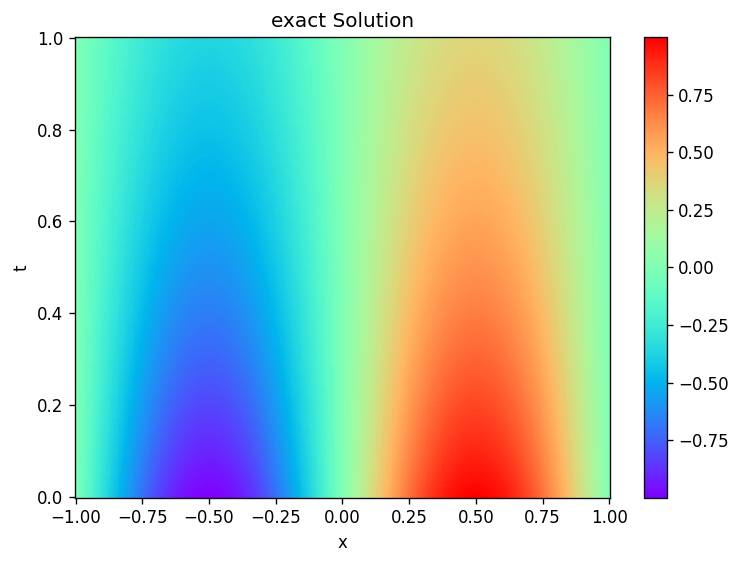
\includegraphics[width=250px]{images/exact_solution_diff.png}
    \vspace{-1em}
    \caption{Exact solution $u(x,t)$}
    \label{exact diff}
\end{figure}

\begin{figure}[H]
    \centering
    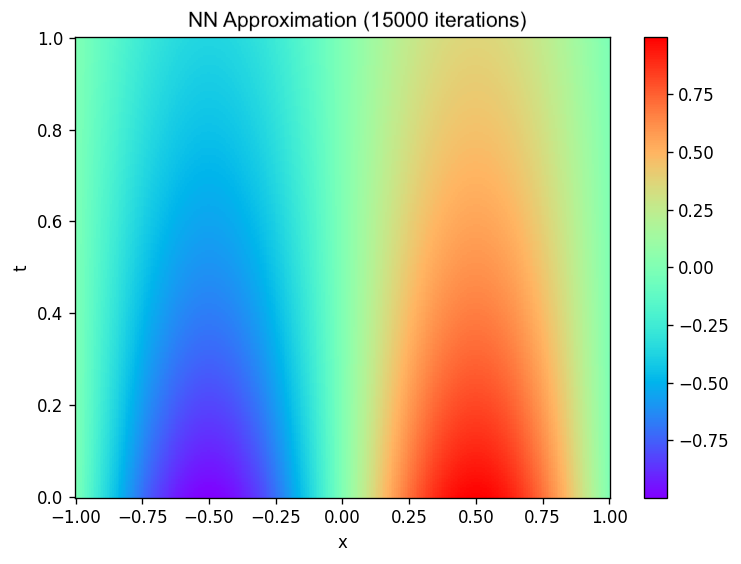
\includegraphics[width=250px]{images/approx_solution_diff.png}
    \vspace{-1em}
    \caption{Approximated solution $u_\theta(x,t)$}
    \label{approximation diff}
\end{figure}

\begin{figure}[H]
    \centering
    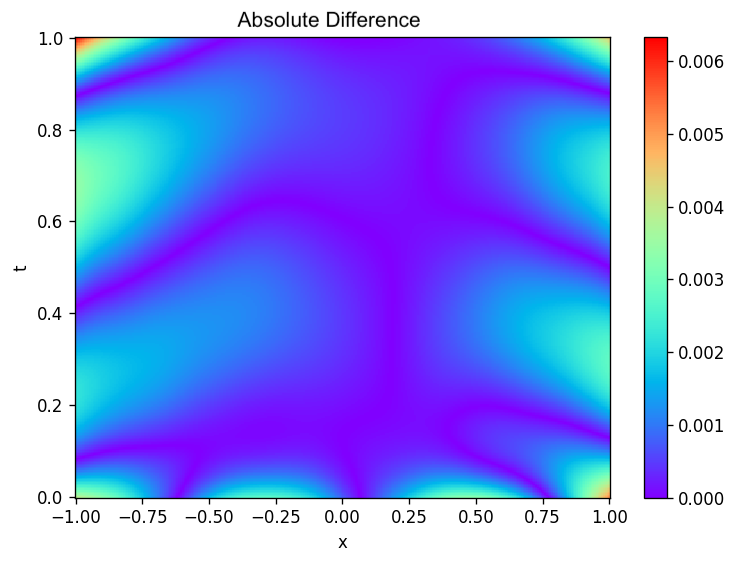
\includegraphics[width=250px]{images/difference_diff.png}
    \vspace{-1em}
    \caption{Absolute difference between $u_(x,t)$ and $u_\theta(x,t)$}
    \label{absolute diff}
\end{figure}

Figure \ref{absolute diff} shows the difference between the exact solution 
in Figure \ref{exact diff} and the neural network approximation in Figure \ref{approximation diff}
where it indicates a global error of order $10^-2$ after 15000 iterations.

\newpage
\section*{Outlines}
\begin{itemize}
    {\item \textbf{Literature Review} {\footnotesize(partially done)}}

    Searching the literature to get a better and clearer understanding of the theoretical 
    and the applied aspects of the topic. This will also help us to determine a relevant industrial problem.

    {\item \textbf{Establishing Connection with Industry}
    {\footnotesize(in progress)}}

    We are currently trying to contact potential companies and organization in order get an industrial 
    support and insight for the project. We are also, trying to find suitable industrial advisor 
    that has an experience in the related field.

    {\item \textbf{Reproducing Previous work} {\footnotesize(partially done)}}

    In order to deepen our understanding of the topic and have more confidence in our work and implementation, 
    we are trying to produce some the previous work in the literature.

    {\item \textbf{Solving the Main problem }}
    
    At this stage, we should be able to apply the skills and the methods that 
    we have searched about and developed to solve the industrial problem.

     {\item \textbf{Validating the Results }}

     After solving the problem, we need to validate our results by analyzing the obtained data.

    {\item \textbf{Demonstration}} 

    Preparing a demonstration to advertise or show the applicability of the project to solve actual problems. 
    This also includes preparing a poster, a report, and a presentation.

    {\item \textbf{Submitting the Project}} 
    
    At this stage, we should make a final review and corrections if necessary before the final submission. 
\end{itemize}

%-------references------
\newpage
\singlespacing
\bibliographystyle{plain}
\bibliography{ref.bib}
 

\end{document}
